\documentclass[preview]{standalone}
\usepackage{amssymb, amsthm}
\usepackage[fleqn]{amsmath}



\usepackage[no-math]{fontspec}
\usepackage{unicode-math}

\setsansfont{texgyreheros}[ 
Extension = {.otf}, 
UprightFont = {*-regular}, 
ItalicFont = {*-italic}, 
BoldFont = {*-bold}, 
BoldItalicFont = {*-bolditalic}] 
%\setmathfont{Stix Two Math}

\usepackage{polyglossia}
\setmainlanguage[babelshorthands=true]{german}
\usepackage[german=guillemets]{csquotes}
\usepackage{microtype}

\usepackage{xcolor}
\definecolor{itwm_blue_04}{RGB}{0,90,148}
\definecolor{background}{RGB}{249,249,249}
\definecolor{my_red}{RGB}{230,0,0}

\usepackage{tikz}
\usepackage{pgfplots}
\pgfplotsset{compat=newest}
\usetikzlibrary{backgrounds}
\usepgfplotslibrary{fillbetween}

\begin{document}
% x   | v(x)
% 1.0 = 50.0
% 1.5 = 49.7
% 2.0 = 48.9
% 2.5 = 47.5
% 3.0 = 45.7
% 3.5 = 43.7
% 4.0 = 41.8
% 4.5 = 40.4
% 5.0 = 40.0
% 5.5 = 41.3
% 6.0 = 45.0

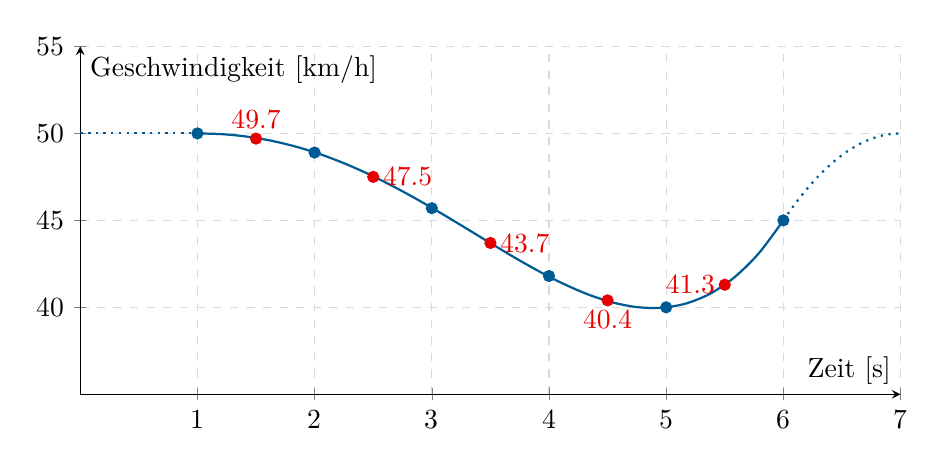
\begin{tikzpicture}background rectangle/.style=
{fill=background,rounded corners=1ex}, show background rectangle]
\begin{axis}[
    domain=1:6,
    axis lines = center,
    xlabel = {Zeit [s]},
    ylabel = {Geschwindigkeit [km/h]},
    height=6cm, width=12cm, 
    xmin=0, xmax=7, ymin=35, ymax=55, 
    xtick={0,1,...,7},
    ytick={35, 40, ...,55},
    grid=major,
    grid style={dashed, gray!30},
]
\path [name path=xaxis]
      (\pgfkeysvalueof{/pgfplots/xmin},0) --
      (\pgfkeysvalueof{/pgfplots/xmax},0);
\addplot[draw=itwm_blue_04, domain=0:1, dotted, smooth, thick, name path=left]{50.0};
\addplot[draw=itwm_blue_04, domain=1:6, smooth, thick, name path=f]{1/10520*(711*x^4-4772*x^3-189*x^2+11850*x+518400)};
\addplot[draw=itwm_blue_04, domain=6:7, dotted, smooth, thick, name path=left]{-5*x^2+70*x-195};
\addplot[color=itwm_blue_04,only marks,mark=*] coordinates{(1,50)(2, 48.9)(3,45.7)(4,41.8)(5, 40.0)(6, 45)};
\addplot[color=my_red,only marks,mark=*] coordinates{(1.5,49.7)} node[above]{49.7};
\addplot[color=my_red,only marks,mark=*] coordinates{(2.5, 47.5)} node[right]{47.5};
\addplot[color=my_red,only marks,mark=*] coordinates{(3.5,43.7)} node[above, right]{43.7};
\addplot[color=my_red,only marks,mark=*] coordinates{(4.5,40.4)} node[left, below]{40.4};
\addplot[color=my_red,only marks,mark=*] coordinates{(5.5, 41.3)} node[above, left]{41.3};

\end{axis}
\end{tikzpicture}


\end{document}